\documentclass{article}

% Input packages & formatting
% Packages

% Math packages
\usepackage{amsmath} % Extended math functions
\usepackage{amssymb} % Extended math symbols (loads in amsfonts)
\usepackage{bm} % Bold math symbols
\usepackage{mathtools}

% Figure packages
\usepackage{caption} % Caption formatting for university standard
\usepackage{graphicx} % includegraphics command
\usepackage{subcaption} % Subfigures
\usepackage[section]{placeins} % Place floats in section
\usepackage{wrapfig}

% Table packages
\usepackage{booktabs} % Better tables
\usepackage{bigstrut} % Merged table cells
\usepackage{longtable} % Tables which overflow into next page
\usepackage{array}
\usepackage{colortbl} % Color table cells
\usepackage{makecell}
\usepackage{multirow}

% Fonts
\usepackage{lmodern} % Use latin modern rather than computer modern. Better for font encoding.
\usepackage[T1]{fontenc} % Allow text to be searchable in output

% Other packages
\usepackage{appendix} % Appendix environment
\usepackage{nextpage} % Cleartooddpage command
%\usepackage[square,comma,sort,numbers]{natbib} % Reference formatting
\usepackage{setspace} % Line spacing
\usepackage{listings} % Display code with syntax highlighting
\usepackage{upquote} % Vertical quotes in verbatim
\usepackage{xcolor} % Colors
\usepackage{titlesec} % Header spacing
\usepackage{xparse} % for tcolorbox
\usepackage[listings]{tcolorbox} % Colored boxes for highlighting syntax
\tcbuselibrary{breakable}
\tcbuselibrary{skins}
\usepackage{enumitem} % better enumerate/itemize options
\usepackage{fancyhdr}
\usepackage{multicol}
\usepackage{ifthen}
\usepackage{xstring}

% Table of contents
\usepackage{imakeidx} % Index page
\usepackage{tocloft} % Control of table of contents
\usepackage[nottoc]{tocbibind} % Adds bibliography, table of tables, table of figures, to table of contents
\usepackage[bookmarks,linktocpage,hidelinks]{hyperref} % Hyperlinks for sections, figures, etc.

% Formatting
% Page format
\setlength{\oddsidemargin}{0.00in}  % Left side margin for odd numbered pages
\setlength{\evensidemargin}{0.00in} % Right side margin for even numbered pages
\setlength{\topmargin}{0.00in}      % Top margin
\setlength{\headheight}{0.20in}     % Header height
\setlength{\headsep}{0.20in}        % Separation between header and main text
\setlength{\topskip}{0.00in}        % Top skip
\setlength{\textwidth}{6.50in}      % Width of the text
\setlength{\textheight}{8.50in}     % Height of the text
\setlength{\footskip}{0.50in}       % Foot skip
\setlength{\parindent}{0.00in}      % First line indentation
\setlength{\parskip}{6pt}        % Space between two paragraphs

% Captions (figures, tables, etc.)
\setlength{\floatsep}{\parskip}          % Space left between floats.
\setlength{\textfloatsep}{\floatsep}   % Space between last top float
% or first bottom float and the text
\setlength{\intextsep}{\floatsep}      % Space left on top and bottom
% of an in-text float
\setlength{\abovecaptionskip}{0.1in plus 0.25in}  % Space above caption
\setlength{\belowcaptionskip}{0.1in plus 0.25in}  % Space below caption
\setlength{\captionmargin}{0.50in}     % Left/Right margin for caption
\setlength{\abovedisplayskip}{0.00in plus 0.25in} % Space before Math stuff
\setlength{\belowdisplayskip}{0.00in plus 0.25in} % Space after Math stuff
\setlength{\arraycolsep}{0.10in}       % Gap between columns of an array
\setlength{\jot}{0.10in}                % Gap between multiline equations
\setlength{\itemsep}{0.10in}           % Space between successive items

% Counters (no section numbering)
\setcounter{tocdepth}{3}
\setcounter{secnumdepth}{0}

% Spacing
\setstretch{1.5}

\titlespacing*{\section}{0cm}{6pt}{6pt}[0cm]
\titlespacing*{\subsection}{0cm}{6pt}{6pt}[0cm]
\titlespacing*{\subsubsection}{0cm}{6pt}{6pt}[0cm]

\titleformat{\section}
{\sffamily\huge}{}{0pt}{\titlerule\vspace{-0.2cm}}
\titleformat{\subsection}
{\sffamily\itshape\Large}{}{0pt}{}

% Macro for syntax
\newtcolorbox{syntax}{
    size=small,
    sharp corners,
    colframe=black,
    colback=yellow,
    fontupper=\bfseries\ttfamily
}

% Macro for argument table
\newenvironment{args}{
    \begin{tabular}{>{\bfseries\ttfamily}p{0.25\linewidth} p{0.69\linewidth}}
    }{
    \end{tabular}\par
    \vspace{0.5\baselineskip}
}

% Note: Requires packages "listing", "xcolor", and "textcomp"
\lstdefinelanguage{verbatim}{
    basicstyle=\ttfamily\small,
    xleftmargin=9pt,
    xrightmargin=9pt,
    columns=fullflexible,
    keepspaces=true,
    comment=[l]{\#},
    breaklines=true
}

\lstdefinestyle{verbatim}{
    commentstyle=\color{gray},
}

% Example code
\AtBeginDocument{
\newtcolorbox[blend into=listings]{example}[2][]{
    colback=blue!3!white,
    colframe=black,
    colbacktitle=blue!15!white,
    coltitle=black,
    sharp corners,
    enhanced,
    breakable,
    size=small,
    before upper={
        \setstretch{1.0}\lstset{language=verbatim,style=verbatim}\vspace{3pt}\textsf{\textit{Code:}}
    },
    subtitle style={
        colback=blue!20!white,
        fonttitle=\sffamily
    },
    before lower={
        \setstretch{1.0}\lstset{language=verbatim,style=verbatim}\vspace{3pt}\textsf{\textit{Output:}}
    },
    fonttitle=\sffamily,
    title={#2},
    #1
}
}

% Links to sub and subsub commands - optional boolean argument, default true. if false, only displays subcmd.

% Commands (and command ensembles)
\newcommand{\command}[1]{\protect\hypertarget{#1}{#1}\index{#1}}
\newcommand{\subcommand}[2]{\protect\hypertarget{#1 #2}{#1 #2}\index{#1!#2}}
\newcommand{\cmdlink}[1]{\protect\hyperlink{#1}{\textit{#1}}}
\newcommand{\subcmdlink}[3][1]{\protect\hyperlink{#2 #3}{\ifnum#1=1\relax\textit{#2 #3}\else\textit{#3}\fi}}

% Methods (first arg is class)
\newcommand{\method}[2]{\protect\hypertarget{$#1Obj #2}{\$#1Obj #2}\index{#1 methods!#2}}
\newcommand{\methodlink}[3][1]{\protect\hyperlink{$#2Obj #3}{\ifnum#1=1\relax\textit{\$#2Obj #3}\else\textit{#3}\fi}}

% Macros for figure/table names
\newcommand{\fig}{\figurename\ }
\newcommand{\figs}{\figurename s }
\newcommand{\tbl}{\tablename\ }
\newcommand{\tbls}{\tablename s }
\newcommand{\eq}{Eq. }
\newcommand{\eqs}{Eqs. }
\renewcommand{\lstlistingname}{Example}% Listing -> Example
\renewcommand{\lstlistlistingname}{List of \lstlistingname s}% List of Listings -> List of Examples
\newcommand{\ex}{Example }
\newcommand{\exs}{Examples }
\newcommand{\var}[1]{\texttt{\textbf{\$#1}}}

% Header/footer
\renewcommand{\headrulewidth}{0pt}

% Changes to hyperlinks (URLs)
\renewcommand\UrlFont{\color{blue}\rmfamily}

% New column type 
% https://tex.stackexchange.com/questions/75717/how-can-i-mix-itemize-and-tabular-environments
\newcolumntype{L}{>{\labelitemi~~}l<{}}
\newcommand{\version}{0.3.1}

\renewcommand{\cleartooddpage}[1][]{\ignorespaces} % single side
\newcommand{\caret}{$^\wedge$}

\title{\Huge{N-Dimensional Lists (ndlist)}\\\large Version \version}
\author{Alex Baker\\\small\url{https://github.com/ambaker1/ndlist}}
\date{\small\today}
\makeindex[columns=2,title={Command Index}]
\begin{document}
\maketitle
\begin{abstract}
\begin{center}
The ``ndlist'' package is a pure Tcl implementation of arbitrary rank tensors.

This package is also a \textcolor{blue}{\href{https://github.com/ambaker1/Tin}{Tin}} package, and can be loaded in as shown below:
\end{center}
\begin{example}{Installing and loading ``ndlist''}
\begin{lstlisting}
package require tin 2.0
tin autoadd ndlist https://github.com/ambaker1/ndlist install.tcl
tin import ndlist
\end{lstlisting}
\end{example}
\end{abstract}
\clearpage

\section{1-Dimensional Lists (Vectors)}
Lists are foundational to Tcl, so in addition to providing utilities for ND-lists, this package also provides utilities for working with 1D-lists, or vectors.
\subsection{Range Generator}
The command \cmdlink{range} simply generates a list of integer values. 
This can be used in conjunction with the Tcl \textit{foreach} loop to simplify writing ``for'' loops.
There are two ways of calling this command, as shown below.
\begin{syntax}
\command{range} \$n \\
range \$start \$stop <\$step>
\end{syntax}
\begin{args}
\$n & Number of indices, starting at 0 (e.g. 3 returns 0 1 2). \\
\$start & Starting value. \\
\$stop & Stop value. \\
\$step & Step size. Default 1 or -1, depending on direction of start to stop.
\end{args}
\begin{example}{Integer range generation}
\begin{lstlisting}
puts [range 3]
puts [range 0 2]
puts [range 10 3 -2]
\end{lstlisting}
\tcblower
\begin{lstlisting}
0 1 2
0 1 2
10 8 6 4
\end{lstlisting}
\end{example}
\begin{example}{Simpler for-loop}
\begin{lstlisting}
foreach i [range 3] {
    puts $i
}
\end{lstlisting}
\tcblower
\begin{lstlisting}
0
1
2
\end{lstlisting}
\end{example}
\clearpage
\subsection{Logical Indexing}
The command \cmdlink{find} returns the indices of non-zero elements of a boolean list, or indices of elements that satisfy a given criterion.
Can be used in conjunction with \cmdlink{nget} to perform logical indexing.
\begin{syntax}
\command{find} \$list <\$op \$scalar>
\end{syntax}
\begin{args}
\$list & List of values to compare. \\
\$op & Comparison operator. Default ``!=''. \\
\$scalar & Comparison value. Default 0.
\end{args}
\begin{example}{Filtering a list}
\begin{lstlisting}
set x {0.5 2.3 4.0 2.5 1.6 2.0 1.4 5.6}
puts [nget $x [find $x > 2]]
\end{lstlisting}
\tcblower
\begin{lstlisting}
2.3 4.0 2.5 5.6
\end{lstlisting}
\end{example}
\subsection{Linear Interpolation}
The command \cmdlink{linterp} performs linear 1D interpolation.
Converts input to ``\cmdlink{float}''.
\begin{syntax}
\command{linterp} \$x \$xList \$yList
\end{syntax}
\begin{args}
\$x & Value to query in \texttt{\$xList} \\
\$xList & List of x points, strictly increasing \\
\$yList & List of y points, same length as \texttt{\$xList}
\end{args}
\begin{example}{Linear interpolation}
\begin{lstlisting}
puts [linterp 2 {1 2 3} {4 5 6}]
puts [linterp 8.2 {0 10 20} {2 -4 5}]
\end{lstlisting}
\tcblower
\begin{lstlisting}
5.0
-2.92
\end{lstlisting}
\end{example}
\clearpage
\subsection{Vector Generation}
The command \cmdlink{linspace} can be used to generate a vector of specified length and equal spacing between two specified values. 
Converts input to ``\cmdlink{float}''
\begin{syntax}
\command{linspace} \$n \$start \$stop 
\end{syntax}
\begin{args}
\$n & Number of points \\
\$start & Starting value \\
\$stop & End value
\end{args}
\begin{example}{Linearly spaced vector generation}
\begin{lstlisting}
puts [linspace 5 0 1]
\end{lstlisting}
\tcblower
\begin{lstlisting}
0.0 0.25 0.5 0.75 1.0
\end{lstlisting}
\end{example}
The command \cmdlink{linsteps} generates intermediate values given an increment size and a sequence of targets.
Converts input to ``\cmdlink{float}''.
\begin{syntax}
\command{linsteps} \$step \$x1 \$x2 ...
\end{syntax}
\begin{args}
\$step & Maximum step size \\
\$x1 \$x2 ... & Targets to hit.
\end{args}
\begin{example}{Intermediate value vector generation}
\begin{lstlisting}
puts [linsteps 0.25 0 1 0]
\end{lstlisting}
\tcblower
\begin{lstlisting}
0.0 0.25 0.5 0.75 1.0 0.75 0.5 0.25 0.0
\end{lstlisting}
\end{example}

\clearpage
\subsection{Functional Mapping}
The command \cmdlink{lapply} simply applies a command over each element of a list, and returns the result.
Basic math operators can be mapped over a list with the command \cmdlink{lop}.
\begin{syntax}
\command{lapply} \$command \$list \$arg ...
\end{syntax}
\begin{syntax}
\command{lop} \$list \$op \$arg... 
\end{syntax}
\begin{args}
\$list & List to map over. \\
\$command & Command prefix to map with. \\
\$op & Math operator (see ::tcl::mathop documentation). \\
\$arg ... & Additional arguments to append to command after each list element. 
\end{args}

\begin{example}{Applying a math function to a list}
\begin{lstlisting}
# Add Tcl math functions to the current namespace path
namespace path [concat [namespace path] ::tcl::mathfunc]
puts [lapply abs {-5 1 2 -2}]
\end{lstlisting}
\tcblower
\begin{lstlisting}
5 1 2 2
\end{lstlisting}
\end{example}

\clearpage
\subsection{Mapping Over Two Lists}
The commands \cmdlink{lapply} and \cmdlink{lop} only map over one list.
The commands \cmdlink{lapply2} and \cmdlink{lop2} allow you to map, element-wise, over two lists.
List lengths must be equal. 
\begin{syntax}
\command{lapply2} \$command \$list1 \$list2 \$arg ...
\end{syntax}
\begin{syntax}
\command{lop2} \$list1 \$op \$list2 \$arg... 
\end{syntax}
\begin{args}
\$list1 \$list2 & Lists to map over, element-wise. \\
\$command & Command prefix to map with. \\
\$op & Math operator (see ::tcl::mathop documentation). \\
\$arg ... & Additional arguments to append to command after list elements. \\
\end{args}

\begin{example}{Mapping over two lists}
\begin{lstlisting}
lapply puts [lapply2 {format "%s %s"} {hello goodbye} {world moon}]
\end{lstlisting}
\tcblower
\begin{lstlisting}
hello world
goodbye moon
\end{lstlisting}
\end{example}

\begin{example}{Adding two lists together}
\begin{lstlisting}
puts [lop2 {1 2 3} + {2 3 2}]
\end{lstlisting}
\tcblower
\begin{lstlisting}
3 5 5
\end{lstlisting}
\end{example}

\clearpage
\subsection{List Statistics}
The commands \cmdlink{max}, \cmdlink{min}, \cmdlink{sum}, \cmdlink{product}, \cmdlink{mean}, \cmdlink{median}, \cmdlink{stdev} and \cmdlink{pstdev} compute the maximum, minimum, sum, product, mean, median, sample and population standard deviation of values in a list.
For more advanced statistics, check out the Tcllib math::statistics package.
\begin{syntax}
\command{max} \$list 
\end{syntax}
\begin{syntax}
\command{min} \$list 
\end{syntax}
\begin{syntax}
\command{sum} \$list
\end{syntax}
\begin{syntax}
\command{product} \$list
\end{syntax}
\begin{syntax}
\command{mean} \$list 
\end{syntax}
\begin{syntax}
\command{median} \$list 
\end{syntax}
\begin{syntax}
\command{stdev} \$list
\end{syntax}
\begin{syntax}
\command{pstdev} \$list
\end{syntax}
\begin{args}
\$list & List to compute statistic of. \\
\end{args}
\begin{example}{List Statistics}
\begin{lstlisting}
set list {-5 3 4 0}
foreach stat {max min sum product mean median stdev pstdev} {
    puts [list $stat [$stat $list]]
}
\end{lstlisting}
\tcblower
\begin{lstlisting}
max 4
min -5
sum 2
product 0
mean 0.5
median 1.5
stdev 4.041451884327381
pstdev 3.5
\end{lstlisting}
\end{example}
\clearpage
\subsection{Vector Algebra}
The dot product of two equal length vectors can be computed with \cmdlink{dot}.
The cross product of two vectors of length 3 can be computed with \cmdlink{cross}. 
\begin{syntax}
\command{dot} \$a \$b
\end{syntax}
\begin{syntax}
\command{cross} \$a \$b
\end{syntax}
\begin{args}
\$a & First vector. \\
\$b & Second vector.
\end{args}
\begin{example}{Dot and cross product}
\begin{lstlisting}
set x {1 2 3}
set y {-2 -4 6}
puts [dot $x $y]
puts [cross $x $y]
\end{lstlisting}
\tcblower
\begin{lstlisting}
8
24 -12 0
\end{lstlisting}
\end{example}
The norm, or magnitude, of a vector can be computed with \cmdlink{norm}.
\begin{syntax}
\command{norm} \$a <\$p>
\end{syntax}
\begin{args}
\$a & Vector to compute norm of. \\
\$p & Norm type. 1 is sum of absolute values, 2 is euclidean distance, and Inf is absolute maximum value. Default 2.
\end{args}
\begin{example}{Normalizing a vector}
\begin{lstlisting}
set x {3 4}
set x [lop $x / [norm $x]]
puts $x
\end{lstlisting}
\tcblower
\begin{lstlisting}
0.6 0.8
\end{lstlisting}
\end{example}
For more advanced vector algebra routines, check out the Tcllib math::linearalgebra package.

\clearpage

\section{2-Dimensional Lists (Matrices)}
A matrix is a two-dimensional list, or a list of row vectors.
This is consistent with the format used in the Tcllib math::linearalgebra package.
See the example below for how matrices are interpreted.
\begin{equation*}\label{eq:matrix_AB}
A=\begin{bmatrix}
2 & 5 & 1 & 3 \\
4 & 1 & 7 & 9 \\
6 & 8 & 3 & 2 \\
7 & 8 & 1 & 4
\end{bmatrix},\quad
B=\begin{bmatrix}
9 \\ 3 \\ 0 \\ -3
\end{bmatrix},\quad
C = \begin{bmatrix}
3 & 7 & -5 & -2
\end{bmatrix}
\end{equation*}
\begin{example}{Matrices and vectors}
\begin{lstlisting}
# Define matrices, column vectors, and row vectors
set A {{2 5 1 3} {4 1 7 9} {6 8 3 2} {7 8 1 4}}
set B {9 3 0 -3}
set C {{3 7 -5 -2}}
# Print out matrices (join with newline to print out each row)
puts "A ="
puts [join $A \n]
puts "B ="
puts [join $B \n]
puts "C ="
puts [join $C \n]
\end{lstlisting}
\tcblower
\begin{lstlisting}
A =
2 5 1 3
4 1 7 9
6 8 3 2
7 8 1 4
B =
9
3
0
-3
C =
3 7 -5 -2
\end{lstlisting}
\end{example}
\clearpage
\subsection{Combining Matrices}
The commands \cmdlink{stack} and \cmdlink{augment} can be used to combine matrices, row or column-wise.
\begin{syntax}
\command{stack} \$mat1 \$mat2 ...
\end{syntax}
\begin{syntax}
\command{augment} \$mat1 \$mat2 ...
\end{syntax}
\begin{args}
\$mat1 \$mat2 ... & Arbitrary number of matrices to stack/augment (number of columns/rows must match)
\end{args}
The command \cmdlink{block} combines a matrix of matrices into a block matrix.
\begin{syntax}
\command{block} \$matrices
\end{syntax}
\begin{args}
\$matrices & Matrix of matrices.
\end{args}
\begin{example}{Combining matrices}
\begin{lstlisting}
set A [stack {{1 2}} {{3 4}}]
set B [augment {1 2} {3 4}]
set C [block [list [list $A $B] [list $B $A]]]
puts $A
puts $B
puts [join $C \n]; # prints each row on a new line
\end{lstlisting}
\tcblower
\begin{lstlisting}
{1 2} {3 4}
{1 3} {2 4}
1 2 1 3
3 4 2 4
1 3 1 2
2 4 3 4
\end{lstlisting}
\end{example}
\clearpage
\subsection{Matrix Transpose}
The command \cmdlink{transpose} simply swaps the rows and columns of a matrix. 
\begin{syntax}
\command{transpose} \$A
\end{syntax}
\begin{args}
\$A & Matrix to transpose, nxm.
\end{args}
Returns an mxn matrix.
\begin{example}{Transposing a matrix}
\begin{lstlisting}
puts [transpose {{1 2} {3 4}}]
\end{lstlisting}
\tcblower
\begin{lstlisting}
{1 3} {2 4}
\end{lstlisting}
\end{example}
\subsection{Matrix Multiplication}
The command \cmdlink{matmul} performs matrix multiplication for two matrices.
Inner dimensions must match.
\begin{syntax}
\command{matmul} \$A \$B
\end{syntax}
\begin{args}
\$A & Left matrix, nxq. \\
\$B & Right matrix, qxm. 
\end{args}
Returns an nxm matrix (or the corresponding dimensions from additional matrices)
\begin{example}{Multiplying a matrix}
\begin{lstlisting}
puts [matmul {{2 5 1 3} {4 1 7 9} {6 8 3 2} {7 8 1 4}} {9 3 0 -3}]
\end{lstlisting}
\tcblower
\begin{lstlisting}
24 12 72 75
\end{lstlisting}
\end{example}
\clearpage
\subsection{Miscellaneous Linear Algebra Routines}
The command \cmdlink{eye} generates an identity matrix.
\begin{syntax}
\command{eye} \$n
\end{syntax}
\begin{args}
\$n  & Size of identity matrix 
\end{args}

The command \cmdlink{outerprod} takes the outer product of two vectors, $\bm{a} \otimes \bm{b} = \bm{a}\bm{b}^T$.
\begin{syntax}
\command{outerprod} \$a \$b
\end{syntax}
\begin{args}
\$a \$b & Vectors with lengths n and m. Returns a matrix, shape nxm.
\end{args}

The command \cmdlink{kronprod} takes the Kronecker product of two matrices, as shown in \eq\eqref{eq:kronprod}.
\begin{syntax}
\command{kronprod} \$A \$B
\end{syntax}
\begin{args}
\$A \$B & Matrices, shapes nxm and pxq. Returns a matrix, shape (np)x(mq).
\end{args}

\begin{equation}\label{eq:kronprod}
\bm{A} \otimes \bm{B} = \left[\begin{matrix}
a_{11}\bm{B} & ... & a_{1n}\bm{B} \\
\vdots & \ddots & \vdots \\
a_{n1}\bm{B} & ... & a_{nn}\bm{B}
\end{matrix}\right]
\end{equation}
\begin{example}{Outer product and Kronecker product}
\begin{lstlisting}
set A [eye 3]
set B [outerprod {1 2} {3 4}]
set C [kronprod $A $B]
puts [join $C \n]; # prints out each row on a new line
\end{lstlisting}
\tcblower
\begin{lstlisting}
3 4 0 0 0 0
6 8 0 0 0 0
0 0 3 4 0 0
0 0 6 8 0 0
0 0 0 0 3 4
0 0 0 0 6 8
\end{lstlisting}
\end{example}
For more advanced matrix algebra routines, check out the Tcllib math::linearalgebra package.
\clearpage
\subsection{Iteration Tools}
The commands \cmdlink{zip} zips two lists into a list of tuples, and \cmdlink{zip3} zip three lists into a list of triples. 
Lists must be the same length.
\begin{syntax}
\command{zip} \$a \$b
\end{syntax}
\begin{syntax}
\command{zip3} \$a \$b \$c
\end{syntax}
\begin{args}
\$a \$b \$c & Lists to zip together.
\end{args}
\begin{example}{Zipping and unzipping lists}
\begin{lstlisting}
# Zipping
set x [zip {A B C} {1 2 3}]
set y [zip3 {Do Re Mi} {A B C} {1 2 3}]
puts $x
puts $y
# Unzipping (using transpose)
puts [transpose $x]
\end{lstlisting}
\tcblower
\begin{lstlisting}
{A 1} {B 2} {C 3}
{Do A 1} {Re B 2} {Mi C 3}
{A B C} {1 2 3}
\end{lstlisting}
\end{example}
The command \cmdlink{cartprod} computes the Cartesian product of an arbitrary number of vectors, returning a matrix where the columns correspond to the input vectors and the rows correspond to all the combinations of the vector elements.
\begin{syntax}
\command{cartprod} \$a \$b ...
\end{syntax}
\begin{args}
\$a \$b ... & Arbitrary number of vectors to take Cartesian product of.
\end{args}

\begin{example}{Cartesian product}
\begin{lstlisting}
puts [cartprod {A B C} {1 2 3}]
\end{lstlisting}
\tcblower
\begin{lstlisting}
{A 1} {A 2} {A 3} {B 1} {B 2} {B 3} {C 1} {C 2} {C 3}
\end{lstlisting}
\end{example}

\clearpage
\section{N-Dimensional Lists (Tensors)}
All Tcl values are ND-lists. An ND-list is defined as a list of equal length (N-1)D-lists, which are defined as equal length (N-2)D-lists, and so on until 0D-lists, which are simply strings that either have no list representation or are of list length 1.
This definition is flexible, and allows for different interpretations of the same data. 
For example, the list ``1 2 3'' can be interpreted as a scalar with value ``1 2 3'', a vector with values ``1'', ``2'', and ``3'', or a matrix with row vectors ``1'', ``2'', and ``3''. 
In general, if a value is a valid for N dimensions, it will also be valid for dimensions 0 to N-1.

The command \cmdlink{ndims} returns the rank of an ND-list, and the command \cmdlink{ndims\_multiple} returns the rank that is compatible with multiple ND-lists. 
By default, it automatically determines the rank for the data, but if a rank is provided, it will validate that the ND-list or ND-lists are compatible with the provided rank. 
\begin{syntax}
\command{ndims} \$ndlist <\$rank>
\end{syntax}
\begin{syntax}
\command{ndims\_multiple} \$ndlists <\$rank>
\end{syntax}
\begin{args}
\$ndlist & ND-list. \\
\$ndlists & List of ND-lists. \\
\$rank & Rank of ND-list (e.g. 2 for matrix) or ``auto'' for auto-rank. Default ``auto''.
\end{args}

\begin{example}{Rank of an ND-list}
\begin{lstlisting}
set x {1}
set y {1 2 {hello world}}; # note that this is not a valid 2D list
set z {{1 2 3} {4 5 6}}
puts [ndims $x]; # 0
puts [ndims $y]; # 1
puts [ndims $z]; # 2
# the only rank that works for x, y, and z is 1
puts [ndims_multiple [list $x $y $z]]; # 1
\end{lstlisting}
\tcblower
\begin{lstlisting}
0
1
2
1
\end{lstlisting}
\end{example}

\clearpage
\subsection{Shape and Size}
The commands \cmdlink{nshape} and \cmdlink{nsize} return the shape and size of an ND-list, respectively.
The shape is a list of the dimensions, and the size is the product of the shape.
\begin{syntax}
\command{nshape} \$ndlist <\$rank>
\end{syntax}
\begin{syntax}
\command{nsize} \$ndlist <\$rank>
\end{syntax}
\begin{args}
\$ndlist & ND-list to get shape/size of. \\
\$rank & Rank of ND-list (e.g. 2 for matrix) or ``auto'' for auto-rank. Default ``auto''.
\end{args}
\begin{example}{Getting shape and size of an ND-list}
\begin{lstlisting}
# Create a 3D list
set x {{{1 2} {3 4} {5 6}} {{7 8} {9 10} {11 12}}}
# Get the shape and size for different rank interpretations
puts [list [nshape $x] [nsize $x]]; # auto-rank (3)
puts [list [nshape $x 1] [nsize $x 1]]; # rank 1
puts [list [nshape $x 2] [nsize $x 2]]; # rank 2
puts [list [nshape $x 3] [nsize $x 3]]; # rank 3
puts [list [nshape $x 4] [nsize $x 4]]; # rank 4
\end{lstlisting}
\tcblower
\begin{lstlisting}
{2 3 2} 12
2 2
{2 3} 6
{2 3 2} 12
{2 3 2 1} 12
\end{lstlisting}
\end{example}

\clearpage
\subsection{Initialization}
The command \cmdlink{nfull} initializes a valid ND-list of any size filled with a single value.
\begin{syntax}
\command{nfull} \$value \$n ...
\end{syntax}
\begin{args}
\$value & Value to repeat \\
\$n ... & Shape (list of dimensions) of ND-list. 
\end{args}
\begin{example}{Generate ND-list filled with one value}
\begin{lstlisting}
puts [nfull foo 3 2]; # 3x2 matrix filled with "foo"
puts [nfull 0 2 2 2]; # 2x2x2 tensor filled with zeros
\end{lstlisting}
\tcblower
\begin{lstlisting}
{foo foo} {foo foo} {foo foo}
{{0 0} {0 0}} {{0 0} {0 0}}
\end{lstlisting}
\end{example}
The command \cmdlink{nrand} initializes a valid ND-list of any size filled with random values between 0 and 1.
\begin{syntax}
\command{nrand} \$n ...
\end{syntax}
\begin{args}
\$n ... & Shape (list of dimensions) of ND-list. 
\end{args}
\begin{example}{Generate random matrix}
\begin{lstlisting}
expr {srand(0)}; # resets the random number seed (for the example)
puts [nrand 1 2]; # 1x2 matrix filled with random numbers
\end{lstlisting}
\tcblower
\begin{lstlisting}
{0.013469574513598146 0.3831388500440581}
\end{lstlisting}
\end{example}
\clearpage
\subsection{Repeating and Expanding}
The command \cmdlink{nrepeat} repeats portions of an ND-list a specified number of times.
\begin{syntax}
\command{nrepeat} \$ndlist \$n ...
\end{syntax}
\begin{args}
\$value & Value to repeat \\
\$n ... & Repetitions at each level.
\end{args}
\begin{example}{Repeat elements of a matrix}
\begin{lstlisting}
puts [nrepeat {{1 2} {3 4}} 1 2]
\end{lstlisting}
\tcblower
\begin{lstlisting}
{1 2 1 2} {3 4 3 4}
\end{lstlisting}
\end{example}
The command \cmdlink{nexpand} repeats portions of an ND-list to expand to new dimensions.
New dimensions must be divisible by old dimensions.
For example, 1x1, 2x1, 4x1, 1x3, 2x3 and 4x3 are compatible with 4x3.
\begin{syntax}
\command{nexpand} \$ndlist \$n ...
\end{syntax}
\begin{args}
\$ndlist & ND-list to expand. \\
\$n ... & New shape of ND-list. If -1 is used, it keeps that axis the same.
\end{args}
\begin{example}{Expand an ND-list to new dimensions}
\begin{lstlisting}
puts [nexpand {1 2 3} -1 2]
puts [nexpand {{1 2}} 2 4]
\end{lstlisting}
\tcblower
\begin{lstlisting}
{1 1} {2 2} {3 3}
{1 2 1 2} {1 2 1 2}
\end{lstlisting}
\end{example}
\clearpage
\subsection{Padding and Extending}
The command \cmdlink{npad} pads an ND-list along its axes by a specified number of elements.
\begin{syntax}
\command{npad} \$ndlist \$value \$n ...
\end{syntax}
\begin{args}
\$ndlist & ND-list to pad. \\
\$value & Value to pad with. \\
\$n ... & Number of elements to pad.
\end{args}
\begin{example}{Padding an ND-list with zeros}
\begin{lstlisting}
set a {{1 2 3} {4 5 6} {7 8 9}}
puts [npad $a 0 2 1]
\end{lstlisting}
\tcblower
\begin{lstlisting}
{1 2 3 0} {4 5 6 0} {7 8 9 0} {0 0 0 0} {0 0 0 0}
\end{lstlisting}
\end{example}
The command \cmdlink{nextend} extends an ND-list to a new shape by padding.
\begin{syntax}
\command{nextend} \$ndlist \$value \$n ...
\end{syntax}
\begin{args}
\$ndlist & ND-list to extend. \\
\$value & Value to pad with. \\
\$n ... & New shape of ND-list.
\end{args}
\begin{example}{Extending an ND-list to a new shape with a filler value}
\begin{lstlisting}
set a {hello hi hey howdy}
puts [nextend $a world -1 2]
\end{lstlisting}
\tcblower
\begin{lstlisting}
{hello world} {hi world} {hey world} {howdy world}
\end{lstlisting}
\end{example}
\clearpage
\subsection{Flattening and Reshaping}
The command \cmdlink{nflatten} flattens an ND-list to a vector.
\begin{syntax}
\command{nflatten} \$ndlist <\$rank>
\end{syntax}
\begin{args}
\$ndlist & ND-list to flatten. \\
\$rank & Rank of ND-list (e.g. 2 for matrix) or ``auto'' for auto-rank. Default ``auto''.
\end{args}
\begin{example}{Reshape a matrix to a 3D tensor}
\begin{lstlisting}
set x [nflatten {{1 2 3 4} {5 6 7 8}}]
puts [nreshape $x 2 2 2]
\end{lstlisting}
\tcblower
\begin{lstlisting}
{{1 2} {3 4}} {{5 6} {7 8}}
\end{lstlisting}
\end{example}

The command \cmdlink{nreshape} reshapes a vector into specified dimensions.
Sizes must be compatible.
\begin{syntax}
\command{nreshape} \$vector \$n ...
\end{syntax}
\begin{args}
\$vector & Vector (1D-list) to reshape. \\
\$n ... & Shape (list of dimensions) of ND-list. One axis may be dynamic, denoted with a "*".
\end{args}
\begin{example}{Reshape a vector to a matrix with three columns}
\begin{lstlisting}
puts [nreshape {1 2 3 4 5 6} * 3]
\end{lstlisting}
\tcblower
\begin{lstlisting}
{1 2 3} {4 5 6}
\end{lstlisting}
\end{example}


\clearpage

\subsection{Index Notation}
This package provides generalized N-dimensional list access/modification commands, using an index notation parsed by the command \cmdlink{::ndlist::ParseIndex}, which returns the index type and an index list for the type.
\begin{syntax}
\command{::ndlist::ParseIndex} \$n \$input
\end{syntax}
\begin{args}
\$n & Number of elements in list. \\
\$input & Index input. Options are shown below: \\
\quad : & All indices \\
\quad \$start:\$stop & Range of indices (e.g. 0:4 or 1:end-2).\\
\quad \$start:\$step:\$stop & Stepped range of indices (e.g. 0:2:-2 or 2:3:end). \\
\quad \$iList & List of indices (e.g. \{0 end-1 5\} or 3). \\
\quad \$i* & Single index with a asterisk, ``flattens'' the ndlist (e.g. 0* or end-3*). 
\end{args}
Additionally, indices get passed through the \cmdlink{::ndlist::Index2Integer} command, which converts the inputs ``end'', ``end-integer'', ``integer$\pm$integer'' and negative wrap-around indexing (where -1 is equivalent to ``end'') into normal integer indices.
Note that this command will return an error if the index is out of range.
\begin{syntax}
\command{::ndlist::Index2Integer} \$n \$index
\end{syntax}
\begin{args}
\$n & Number of elements in list. \\
\$index & Single index. 
\end{args}

\begin{example}{Index Notation}
\begin{lstlisting}
set n 10
puts [::ndlist::ParseIndex $n :]
puts [::ndlist::ParseIndex $n 1:8]
puts [::ndlist::ParseIndex $n 0:2:6]
puts [::ndlist::ParseIndex $n {0 5 end-1}]
puts [::ndlist::ParseIndex $n end*]
\end{lstlisting}
\tcblower
\begin{lstlisting}
A {}
R {1 8}
L {0 2 4 6}
L {0 5 8}
S 9
\end{lstlisting}
\end{example}
\clearpage
\subsection{Access}
Portions of an ND-list can be accessed with the command \cmdlink{nget}, using the index parser \cmdlink{::ndlist::ParseIndex} for each dimension being indexed.
Note that unlike the Tcl \textit{lindex} and \textit{lrange} commands, \cmdlink{nget} will return an error if the indices are out of range.
\begin{syntax}
\command{nget} \$ndlist \$i ...
\end{syntax}
\begin{args}
\$ndlist & ND-list value. \\
\$i ... & Index inputs, parsed with \cmdlink{::ndlist::ParseIndex}. 
\end{args}
\begin{example}{ND-list access}
\begin{lstlisting}
set A {{1 2 3} {4 5 6} {7 8 9}}
puts [nget $A 0 :]; # get row matrix
puts [nget $A 0* :]; # flatten row matrix to a vector
puts [nget $A 0:1 0:1]; # get matrix subset
puts [nget $A end:0 end:0]; # can have reverse ranges
puts [nget $A {0 0 0} 1*]; # can repeat indices
\end{lstlisting}
\tcblower
\begin{lstlisting}
{1 2 3}
1 2 3
{1 2} {4 5}
{9 8 7} {6 5 4} {3 2 1}
2 2 2
\end{lstlisting}
\end{example}

\clearpage
\subsection{Modification}
A ND-list can be modified by reference with \cmdlink{nset}, and by value with \cmdlink{nreplace}, using the index parser \cmdlink{::ndlist::ParseIndex} for each dimension being indexed.
Note that unlike the Tcl \textit{lset} and \textit{lreplace} commands, the commands \cmdlink{nset} and \cmdlink{nreplace} will return an error if the indices are out of range.
If all the index inputs are ``\texttt{:}'' except for one, and the replacement list is blank, it will delete values along that axis by calling \cmdlink{nremove}.
Otherwise, the replacement ND-list must be expandable to the target index dimensions. 

If using the ``\texttt{= \$expr}'' notation, it will call \cmdlink{nexpr}, where ``self'' is the ND-list or indexed range being modified and ``rank'' is ``auto'' if no index arguments are provided, otherwise it is equal to the number of index arguments minus the number of single index (S) arguments (see \cmdlink{::ndlist::ParseIndex}).
\begin{syntax}
\command{nset} \$varName \$i ... (\$sublist | = \$expr)
\end{syntax}
\begin{syntax}
\command{nreplace} \$ndlist \$i ... (\$sublist | = \$expr)
\end{syntax}
\begin{args}
\$varName & Variable that contains an ND-list. \\
\$ndlist & ND-list to modify. \\
\$i ... & Index inputs, parsed with \cmdlink{::ndlist::ParseIndex}. \\
\$sublist & Replacement list, or blank to delete values. \\
\$expr & Expression to evaluate and replace values with. Indexed range can be accessed with ``\texttt{@.}'' for convenience.
\end{args}


\begin{example}{ND-list modification}
\begin{lstlisting}
# Swap rows in a matrix (by reference)
set a {{1 2 3} {4 5 6} {7 8 9}}
nset a {1 0} : [nget $a {0 1} :]
puts $a
# Element-wise operation on portion of vector (by value)
set b [range 10]
puts [nreplace $b 0:2:end = {@. + 10}]
\end{lstlisting}
\tcblower
\begin{lstlisting}
{4 5 6} {1 2 3} {7 8 9}
10 1 12 3 14 5 16 7 18 9
\end{lstlisting}
\end{example}
\clearpage

\clearpage
\subsection{Removal}
The command \cmdlink{nremove} removes portions of an ND-list at a specified axis.
\begin{syntax}
\command{nremove} \$ndlist \$i <\$axis>
\end{syntax}
\begin{args}
\$ndlist & ND-list to modify. \\
\$i & Index input, parsed with \cmdlink{::ndlist::ParseIndex}. \\
\$axis & Axis to remove at. Default 0.
\end{args}

\begin{example}{Filtering a list by removing elements}
\begin{lstlisting}
set x [range 10]
puts [nremove $x [find $x > 4]]
\end{lstlisting}
\tcblower
\begin{lstlisting}
0 1 2 3 4
\end{lstlisting}
\end{example}

\begin{example}{Deleting a column from a matrix}
\begin{lstlisting}
set a {{1 2 3} {4 5 6} {7 8 9}}
puts [nremove $a 2 1]
\end{lstlisting}
\tcblower
\begin{lstlisting}
{1 2} {4 5} {7 8}
\end{lstlisting}
\end{example}
\clearpage
\subsection{Insertion and Concatenation}
The command \cmdlink{ninsert} inserts an ND-list into another ND-list at a specified index and axis.
The ND-lists must agree in dimension at all other axes.
If ``end'' or ``end-integer'' is used for the index, it will insert after the index. 
Otherwise, it will insert before the index.
The command \cmdlink{ncat} is shorthand for inserting at ``end'', and concatenates two ND-lists.
\begin{syntax}
\command{ninsert} \$ndlist1 \$index \$ndlist2 <\$axis> <\$rank>
\end{syntax}
\begin{syntax}
\command{ncat} \$ndlist1 \$ndlist2 <\$axis> <\$rank> 
\end{syntax}
\begin{args}
\$ndlist1 \$ndlist2 & ND-lists to combine. \\
\$index & Index to insert at. \\
\$axis & Axis to insert/concatenate at (default 0). \\
\$rank & Rank of ND-list (e.g. 2 for matrix) or ``auto'' for auto-rank. Default ``auto''.
\end{args}

\begin{example}{Inserting a column into a matrix}
\begin{lstlisting}
set matrix {{1 2} {3 4} {5 6}}
set column {A B C}
puts [ninsert $matrix 1 $column 1 2]
\end{lstlisting}
\tcblower
\begin{lstlisting}
{1 A 2} {3 B 4} {5 C 6}
\end{lstlisting}
\end{example}
\begin{example}{Concatenate tensors}
\begin{lstlisting}
set x [nreshape {1 2 3 4 5 6 7 8 9} 3 3 1]
set y [nreshape {A B C D E F G H I} 3 3 1]
puts [ncat $x $y 2 3]
\end{lstlisting}
\tcblower
\begin{lstlisting}
{{1 A} {2 B} {3 C}} {{4 D} {5 E} {6 F}} {{7 G} {8 H} {9 I}}
\end{lstlisting}
\end{example}

\clearpage
\subsection{Changing Order of Axes}
The command \cmdlink{nswapaxes} is a general purpose transposing function that swaps the axes of an ND-list.
For simple matrix transposing, the command \cmdlink{transpose} can be used instead.
\begin{syntax}
\command{nswapaxes} \$ndlist \$axis1 \$axis2
\end{syntax}
\begin{args}
\$ndlist & ND-list to manipulate. \\
\$axis1 \$axis2 & Axes to swap.
\end{args}
The command \cmdlink{nmoveaxis} moves a specified source axis to a target position. 
For example, moving axis 0 to position 2 would change ``i,j,k'' to ``j,k,i''.
\begin{syntax}
\command{nmoveaxis} \$ndlist \$source \$target
\end{syntax}
\begin{args}
\$ndlist & ND-list to manipulate. \\
\$source & Source axis. \\
\$target & Target position.
\end{args}
The command \cmdlink{npermute} is more general purpose, and defines a new order for the axes of an ND-list.
For example, the axis list ``1 0 2'' would change ``i,j,k'' to ``j,i,k''. 
\begin{syntax}
\command{npermute} \$ndlist \$axis ...
\end{syntax}
\begin{args}
\$ndlist & ND-list to manipulate. \\
\$axis ... & List of axes defining new order.
\end{args}
\begin{example}{Changing tensor axes}
\begin{lstlisting}
set x {{{1 2} {3 4}} {{5 6} {7 8}}}
set y [nswapaxes $x 0 2]
set z [nmoveaxis $x 0 2]
puts [lindex $x 0 0 1]
puts [lindex $y 1 0 0]
puts [lindex $z 0 1 0]
\end{lstlisting}
\tcblower
\begin{lstlisting}
2
2
2
\end{lstlisting}
\end{example}

\clearpage
\subsection{ND Functional Mapping}
The command \cmdlink{napply} applies a command over each element of an ND-list, and returns the result.
The commands \cmdlink{napply2} maps element-wise over two ND-lists. 
If the input lists have different shapes, they will be expanded to their maximum dimensions with \cmdlink{nexpand} (if compatible).
\begin{syntax}
\command{napply} \$command \$ndlist <\$suffix> <\$rank>
\end{syntax}
\begin{syntax}
\command{napply2} \$command \$ndlist1 \$ndlist2 <\$suffix> <\$rank> 
\end{syntax}
\begin{args}
\$ndlist & ND-list to map over. \\
\$ndlist1 \$ndlist2 & ND-lists to map over, element-wise. \\
\$command & Command prefix to map with. \\
\$suffix & Additional arguments to append after ND-list elements. Default blank. \\
\$rank & Rank of ND-list (e.g. 2 for matrix) or ``auto'' for auto-rank. Default ``auto''.
\end{args}
\begin{example}{Chained functional mapping over a matrix}
\begin{lstlisting}
napply puts [napply {format %.2f} [napply expr {{1 2} {3 4}} {+ 1}]]
\end{lstlisting}
\tcblower
\begin{lstlisting}
2.00
3.00
4.00
5.00
\end{lstlisting}
\end{example}
\begin{example}{Format columns of a matrix}
\begin{lstlisting}
set data {{1 2 3} {4 5 6} {7 8 9}}
set formats {{%.1f %.2f %.3f}}
puts [napply2 format $formats $data]
\end{lstlisting}
\tcblower
\begin{lstlisting}
{1.0 2.00 3.000} {4.0 5.00 6.000} {7.0 8.00 9.000}
\end{lstlisting}
\end{example}
\clearpage
\subsection{Reducing an ND-list}
The command \cmdlink{nreduce} combines \cmdlink{nmoveaxis} and \cmdlink{napply} to reduce an axis of an ND-list with a function that reduces a vector to a scalar, like \cmdlink{max} or \cmdlink{sum}.
\begin{syntax}
\command{nreduce} \$command \$ndlist <\$axis> <\$suffix> <\$rank>
\end{syntax}
\begin{args}
\$command & Command prefix to map with. \\
\$ndlist & ND-list to map over. \\
\$axis & Axis to reduce. Default 0. \\
\$suffix & Additional arguments to append after ND-list elements. Default blank. \\
\$rank & Rank of ND-list (e.g. 2 for matrix) or ``auto'' for auto-rank. Default ``auto''.
\end{args}
\begin{example}{Matrix row and column statistics}
\begin{lstlisting}
set x {{1 2} {3 4} {5 6} {7 8}}
puts [nreduce max $x]; # max of each column
puts [nreduce max $x 1]; # max of each row
puts [nreduce sum $x]; # sum of each column
puts [nreduce sum $x 1]; # sum of each row
\end{lstlisting}
\tcblower
\begin{lstlisting}
7 8
2 4 6 8
16 20
3 7 11 15
\end{lstlisting}
\end{example}

\clearpage
\subsection{Generalized N-Dimensional Mapping}
The command \cmdlink{nmap} is a general purpose mapping function for N-dimensional lists in Tcl.
If multiple ND-lists are provided for iteration, they must be expandable to their maximum dimensions.
The actual implementation flattens all the ND-lists and calls the Tcl \textit{lmap} command, and then reshapes the result to the target dimensions.
So, if ``continue'' or ``break'' are used in the map body, it will return an error.
If rank is not specified, it will automatically determine the rank using \cmdlink{ndims\_multiple} and the referenced ND-lists.
\begin{syntax}
\command{nmap} <\$rank> \$varName \$ndlist <\$varName \$ndlist ...> \$body
\end{syntax}
\begin{args}
\$rank & Rank (e.g. 2 for matrix) or ``auto'' for auto-rank. Default ``auto''.  \\
\$varName & Variable name to iterate with. \\
\$ndlist & ND-list to iterate over. \\
\$body & Tcl script to evaluate at every loop iteration. 
\end{args}

\begin{example}{Expand and map over matrices}
\begin{lstlisting}
set phrases [nmap 2 greeting {{hello goodbye}} subject {world moon} {
    list $greeting $subject
}]
napply puts $phrases {} 2 
\end{lstlisting}
\tcblower
\begin{lstlisting}
hello world
goodbye world
hello moon
goodbye moon
\end{lstlisting}
\end{example}
\clearpage
\subsection{Loop Index Access}
The iteration indices of \cmdlink{nmap} can be accessed with the commands \cmdlink{i}, \cmdlink{j}, and \cmdlink{k}. 
The commands \cmdlink{j} and \cmdlink{k} are simply shorthand for \cmdlink{i} with axes 1 and 2.
\begin{syntax}
\command{i} <\$axis>
\end{syntax}
\begin{syntax}
\command{j}
\end{syntax}
\begin{syntax}
\command{k}
\end{syntax}
\begin{args}	
\$axis & Dimension to access mapping index at. Default 0. \\
 & If -1, returns the linear index of the loop.
\end{args}

\begin{example}{Finding index tuples that match criteria}
\begin{lstlisting}
set x {{1 2 3} {4 5 6} {7 8 9}}
set indices {}
nmap xi $x {
    if {$xi > 4} {
        lappend indices [list [i] [j]]
    }
}
puts $indices
\end{lstlisting}
\tcblower
\begin{lstlisting}
{1 1} {1 2} {2 0} {2 1} {2 2}
\end{lstlisting}
\end{example}
\clearpage

\subsection{Element-wise operations}
The command \cmdlink{neval} maps over ND-arrays using \cmdlink{nmap}, but without the need to specify looping variables, and the command \cmdlink{nexpr} is a special case that passes input through the Tcl \textit{expr} command.
ND-lists can be referred to with ``\texttt{@ref}'', where ``ref'' is the name of the variable storing the ND-list.
If an ND-list is provided as ``self'', it can be referred to with ``\texttt{@.}'' for convenience.
Additionally, portions of an ND-list can be mapped over with the notation ``\texttt{@ref(\$i,...)}'', where ``\texttt{\$i,...}'' are raw index arguments (does not do any substitution).
If rank is not specified, it will automatically determine the rank using \cmdlink{ndims\_multiple} and the referenced/indexed ND-lists.
\begin{syntax}
\command{neval} \$body <\$self> <\$rank>
\end{syntax}
\begin{syntax}
\command{nexpr} \$expr <\$self> <\$rank>
\end{syntax}
\begin{args}
\$body & Script to evaluate, with ``\texttt{@ref}'' notation for ND-list references. \\
\$expr & Expression to evaluate, with ``\texttt{@ref}'' notation for ND-list references. \\
\$self & ND-list to refer to with ``\texttt{@.}''. Default blank. \\
\$rank & Rank (e.g. 2 for matrix) or ``auto'' for auto-rank. Default ``auto''. 
\end{args}

\begin{example}{Get distance between elements in a vector}
\begin{lstlisting}
set x {1 2 4 7 11 16}
puts [nexpr {@x(1:end) - @x(0:end-1)}]
\end{lstlisting}
\tcblower
\begin{lstlisting}
1 2 3 4 5
\end{lstlisting}
\end{example}

\begin{example}{Outer product of two vectors}
\begin{lstlisting}
set x {1 2 3}
set y {{4 5 6}}
puts [nexpr {@x * @y}]
\end{lstlisting}
\tcblower
\begin{lstlisting}
{4 5 6} {8 10 12} {12 15 18}
\end{lstlisting}
\end{example}



\clearpage
\section{ND-Arrays}
The command \cmdlink{narray} is a TclOO class based on the superclass \textit{::vutil::ValueContainer}, from the package \textcolor{blue}{\href{https://github.com/ambaker1/vutil}{vutil}}. 
It is an object-oriented approach to array manipulation and processing.

\begin{syntax}
\command{narray} new \$nd \$varName <\$ndlist>
\end{syntax}
\begin{syntax}
\command{narray} create \$name \$nd \$varName <\$ndlist>
\end{syntax}
\begin{args}
\$nd & Rank of ND-array (e.g. 2D, 2d, or 2 for a matrix). \\
\$varName & Variable to store object name for access and garbage collection. 
Variable names are restricted to word characters and namespace delimiters only.\\
\$ndlist & ND-list value to store in ND-array. Default blank. \\
\$name & Name of object if using ``create'' method.
\end{args}
\subsection{Value, Rank, Shape, and Size}
The value is accessed by calling the object by itself, the rank is accessed with the method \methodlink[0]{narray}{rank}, and the shape and size are accessed with the methods \methodlink[0]{narray}{shape} and \methodlink[0]{narray}{size}.
\begin{syntax}
\method{narray}{rank}
\end{syntax}
\begin{syntax}
\method{narray}{shape} <\$axis>
\end{syntax}
\begin{syntax}
\method{narray}{size}
\end{syntax}
\begin{args}
\$axis & Axis to get dimension along. Default blank for all axes. \\
\end{args}
\begin{example}{Creating ND-arrays}
\begin{lstlisting}
# Create new ND-arrays
narray new 2D x {{1 2 3} {4 5 6} {7 8 9}}
narray new 1D y {hello world}
# Print rank and value of ND-arrays
puts "[$x rank], [$x]"
puts "[$y rank], [$y]"
\end{lstlisting}
\tcblower
\begin{lstlisting}
2, {1 2 3} {4 5 6} {7 8 9}
1, hello world
\end{lstlisting}
\end{example}

\clearpage
\subsection{Indexing}
The ``\texttt{@}'' operator uses \cmdlink{nget} to access a portion of the ND-array. 
\begin{syntax}
\index{narray methods!@} \$narrayObj @ \$i ...
\end{syntax}
\begin{args}
\$i ... & Index inputs corresponding with rank of ND-array. \\
\end{args}

\begin{example}{Accessing portions of an ND-array}
\begin{lstlisting}
narray new 2D x {{1 2 3} {4 5 6} {7 8 9}}
puts [$x @ 0 2]
puts [$x @ 0:end-1 {0 2}]
\end{lstlisting}
\tcblower
\begin{lstlisting}
3
{1 3} {4 6}
\end{lstlisting}
\end{example}

\subsection{Copying}
The operator ``\texttt{-{}->}'' copies the ND-array to a new variable, and returns the new object.
If indices are specified, the new ND-array object will have the rank of the indexed range.
\begin{syntax}
\index{narray methods!-{}->} \$narrayObj <@ \$i ...> -{}-> \$varName
\end{syntax}
\begin{args}
\$i ... & Indices to access. Default all. \\
\$varName & Variable to store object name for access and garbage collection. 
Variable names are restricted to word characters and namespace delimiters only.
\end{args}

\begin{example}{Copying a portion of an ND-array}
\begin{lstlisting}
narray new 2 x {{1 2 3} {4 5 6}}
$x @ 0* : --> y; # Row vector (flattened to 1D)
puts "[$y rank], [$y]"
\end{lstlisting} 
\tcblower
\begin{lstlisting}
1, 1 2 3
\end{lstlisting}
\end{example}
\clearpage
\subsection{Evaluation/Mapping}
The command \cmdlink{neval} maps over ND-arrays using \cmdlink{nmap}. 
The command \cmdlink{nexpr} is a special case that passes input through the Tcl \textit{expr} command.
ND-arrays can be referred to with ``\texttt{\$@ref}'', where ``ref'' is the name of the ND-array variable.
Portions of an ND-array can be mapped over with the notation ``\texttt{\$@ref(\$i,...)}''.
Input ND-arrays must all agree in rank or be scalar. 
Additionally, they must have compatible dimensions.
\begin{syntax}
\command{neval} \$body <\$self> <\$rankVar>
\end{syntax}
\begin{syntax}
\command{nexpr} \$expr <\$self> <\$rankVar>
\end{syntax}
\begin{args}
\$body & Script to evaluate, with ``\texttt{\$@ref}'' notation for object references. \\
\$expr & Expression to evaluate, with ``\texttt{\$@ref}'' notation for object references. \\
\$self & Object to refer to with ``\texttt{\$@}''. Default blank. \\
\$rankVar & Variable to store resulting rank in. Default blank.
\end{args}

\begin{example}{Get distance between elements in a vector}
\begin{lstlisting}
narray new 1D x {1 2 4 7 11 16}
puts [nexpr {$@x(1:end) - $@x(0:end-1)}]
\end{lstlisting}
\tcblower
\begin{lstlisting}
1 2 3 4 5
\end{lstlisting}
\end{example}

\begin{example}{Outer product of two vectors}
\begin{lstlisting}
narray new 2D x {1 2 3}
narray new 2D y {{4 5 6}}
puts [nexpr {$@x * $@y}]
\end{lstlisting}
\tcblower
\begin{lstlisting}
{4 5 6} {8 10 12} {12 15 18}
\end{lstlisting}
\end{example}

\clearpage
\subsection{Modification}
The assignment operator, ``\texttt{=}'', sets the value of the entire ND-array, or of a specified range.
The math assignment operator, ``\texttt{:=}'', sets the value, passing the input through the \cmdlink{nexpr} command. 
Both assignment operators return the object.

\begin{syntax}
\index{narray methods!=} \$narrayObj <@ \$i ...> = \$value
\end{syntax}
\begin{syntax}
\index{narray methods!:=} \$narrayObj <@ \$i ...> := \$expr
\end{syntax}
\begin{args}
\$i ... & Indices to modify. Default all. \\
\$value & Value to assign. Blank to remove values. \\
\$expr & Expression to evaluate.
\end{args}

If using the math assignment operator, the ND-array or indexed range can be accessed with the alias ``\texttt{\$.}'', and the elements of the array or indexed range can be accessed with ``\texttt{\$@}''.
\begin{syntax}
\$. \$arg ...
\end{syntax}
\begin{args}
\$arg ... & Method arguments for object.
\end{args}

\begin{example}{Element-wise modification of a vector}
\begin{lstlisting}
# Create blank vectors and assign values
[narray new 1D x] = {1 2 3}
[narray new 1D y] = {10 20 30}
# Add one to each element
puts [$x := {$@ + 1}]
# Double the last element
puts [$x @ end := {$@ * 2}]
# Element-wise addition of vectors
puts [$x := {$@ + $@y}]
\end{lstlisting}
\tcblower
\begin{lstlisting}
2 3 4
2 3 8
12 23 38
\end{lstlisting}
\end{example}

\clearpage
\subsection{Removal/Insertion}
The method \methodlink[0]{narray}{remove} removes portions of an ND-array along a specified axis, returning the object.

The method \methodlink[0]{narray}{insert} inserts values into an ND-array at a specified index/axis, returning the object.

\begin{syntax}
\method{narray}{remove} \$index <\$axis>
\end{syntax}
\begin{syntax}
\method{narray}{insert} \$index \$sublist <\$axis>
\end{syntax}
\begin{args}
\$index & Index to remove/insert at. \\
\$sublist & Value to insert. \\
\$axis & Axis to remove/insert at (default 0).
\end{args}

\begin{example}{Removing elements from a vector}
\begin{lstlisting}
narray new 1 vector {1 2 3 4 5 6 7 8}
# Remove all odd numbers
$vector remove [find [nexpr {$@vector % 2}]]
puts [$vector]
\end{lstlisting}
\tcblower
\begin{lstlisting}
2 4 6 8
\end{lstlisting}
\end{example}

\begin{example}{Inserting a column into a matrix}
\begin{lstlisting}
narray new 2 matrix {{1 2} {3 4} {5 6}}
puts [$matrix insert 1 {A B C} 1]
\end{lstlisting}
\tcblower
\begin{lstlisting}
{1 A 2} {3 B 4} {5 C 6}
\end{lstlisting}
\end{example}


\clearpage
\subsection{Map/Reduce}
The method \methodlink[0]{narray}{apply} maps a command over the ND-array, returning the value, and the method \methodlink[0]{narray}{reduce} applies a reducing command over a specified axis, returning the value. 
Both commands do not modify the object.

\begin{syntax}
\method{narray}{apply} \$command \$arg ...
\end{syntax}
\begin{syntax}
\method{narray}{reduce} \$command <\$axis> \$arg ...
\end{syntax}
\begin{args}
\$command & Command prefix to map over the ND-list object. \\
\$arg ... & Additional arguments to append to command. \\
\$axis & Axis to reduce at (default 0).
\end{args}

\begin{example}{Map a command over a list}
\begin{lstlisting}
narray new 1 text {The quick brown fox jumps over the lazy dog}
puts [$text apply {string length}]; # Print the length of each word
\end{lstlisting}
\tcblower
\begin{lstlisting}
3 5 5 3 5 4 3 4 3
\end{lstlisting}
\end{example}

\begin{example}{Get column statistics of a matrix}
\begin{lstlisting}
narray new 2 matrix {{1 2 3} {4 5 6} {7 8 9}}
# Convert to double-precision floating point
$matrix = [$matrix apply ::tcl::mathfunc::double]
# Get maximum and minimum of each column
puts [$matrix reduce max 1]
puts [$matrix reduce min 1]
\end{lstlisting}
\tcblower
\begin{lstlisting}
7.0 8.0 9.0
1.0 2.0 3.0
\end{lstlisting}
\end{example}

\clearpage
\subsection{Temporary Object Evaluation}
The pipe operator, ``\texttt{|}'', copies the ND-array to a temporary object, and evaluates the method.
Returns the result of the method, or the value of the temporary object.
This operator is useful for converting methods that modify the object to methods that return a modified value.
\begin{syntax}
\index{narray methods!$\vert$} \$narrayObj <@ \$i ...> | \$method \$arg ...
\end{syntax}
\begin{args}
\$i ... & Indices to access. Default all. \\
\$method & Method to evaluate. \\
\$arg ... & Arguments to pass to method.
\end{args}
\begin{example}{Temporary object value}
\begin{lstlisting}
# Create a matrix
narray new 2 x {{1 2 3} {4 5 6}}
# Print value with first row doubled.
puts [$x | @ 0* : := {$@ * 2}]
# Source object was not modified
puts [$x]
\end{lstlisting} 
\tcblower
\begin{lstlisting}
{2 4 6} {4 5 6}
{1 2 3} {4 5 6}
\end{lstlisting}
\end{example}
\clearpage
\subsection{Reference Variable Evaluation}
The operator ``\texttt{\&}'' copies the ND-array value or range to a reference variable, and evaluates a body of script. 
The changes made to the reference variable will be applied to the object, and if the variable is unset, the object will be deleted.
If no indices are specified and the variable is unset in the script, the ND-array object will be destroyed.
Returns the result of the script.

\begin{syntax}
\index{narray methods!\&} \$narrayObj <@ \$i ...> \& \$refName \$body
\end{syntax}
\begin{args}
\$i ... & Indices to access. Default all. \\
\$refName & Variable name to use for reference. \\
\$body & Body to evaluate.
\end{args}

\begin{example}{Appending a vector}
\begin{lstlisting}
# Create a 1D list
narray new 1 x {1 2 3}
# Append the list
$x & ref {lappend ref 4 5 6}
puts [$x]
# Append a subset of the list
$x @ end & ref {lappend ref 7 8 9}
puts [$x]
\end{lstlisting}
\tcblower
\begin{lstlisting}
1 2 3 4 5 6
1 2 3 4 5 {6 7 8 9}
\end{lstlisting}
\end{example}

\clearpage





\section{Tabular Data Structure}
This package also provides support for a tabular datatype.
The string representation of the table datatype is a matrix, with the first row being the header.
The values in the first column must be unique, and are called the table's ``keys''. 
Correspondingly, the first header entry is called the ``keyname'', and the remaining header entries are the table's ``fields''. 
The rest of the matrix is the table's data, accessible by indexing with keys and fields.
Missing values are represented by blanks.
The conceptual layout of the table is illustrated in the figure below.
\vspace{\baselineskip}
\FloatBarrier
\begin{figure}[!htb]
    \centering
    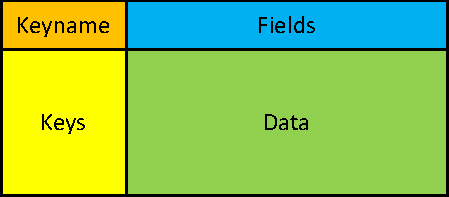
\includegraphics{figures/table.pdf}
    \caption{Conceptual Representation of Tabular Data Structure}
    \label{fig:table_props}
\end{figure}

The command \cmdlink{table} is a TclOO class based on the superclass \textit{::vutil::ValueContainer}, from the package \textcolor{blue}{\href{https://github.com/ambaker1/vutil}{vutil}}. 
It is an object-oriented approach to tabular data manipulation.
\begin{syntax}
\command{table} new \$varName <\$value>
\end{syntax}
\begin{syntax}
table create \$name \$varName <\$value>
\end{syntax}
\begin{args}
\$varName & Variable to store object name for access and garbage collection.  \\
\$value & Matrix representation of table. Default blank. \\
\$name & Name of object if using ``create'' method.
\end{args}

\begin{example}{Creating and accessing a table}
\begin{lstlisting}
table new tableObj {{key A B} {1 foo bar} {2 hello world}}
puts [$tableObj]
\end{lstlisting}
\tcblower
\begin{lstlisting}
{key A B} {1 foo bar} {2 hello world}
\end{lstlisting}
\end{example}


\clearpage

\subsection{Basic Operators}
Because the table class is a subclass of \textit{::vutil::ValueContainer}, it has the same operator methods. 

The copy operator, ``\texttt{-{}->}'', copies the table to a new variable, and returns the new object.
\begin{syntax}
\index{table methods!-{}->} \$tableObj -{}-> \$varName
\end{syntax} 
\begin{args}
\$varName & Variable to store object name for access and garbage collection. 
\end{args}

The assignment operator, ``\texttt{=}'', sets the value of the entire table, and the math assignment operator, ``\texttt{:=}'', sets the value after passing the input through the Tcl \textit{expr} command. 
Both operators return the object.

\begin{syntax}
\index{table methods!=} \$tableObj = \$value
\end{syntax}
\begin{syntax}
\index{table methods!:=} \$tableObj := \$expr
\end{syntax}

\begin{args}
\$value & Value to assign. \\
\$expr & Expression to evaluate.
\end{args}

The pipe operator, ``\texttt{|}'', copies the table to a temporary object, and evaluates the method.
Returns the result of the method, or the value of the temporary object.
This operator is useful for converting methods that modify the object to methods that return a modified value.

\begin{syntax}
\index{table methods!$\vert$} \$tableObj | \$method \$arg ...
\end{syntax}

\begin{args}
\$method & Method to evaluate. \\
\$arg ... & Arguments to pass to method.
\end{args}

The ampersand operator ``\texttt{\&}'' copies the table value to a reference variable, and evaluates a body of script. 
The changes made to the reference variable will be applied to the object, and if the variable is unset, the object will be deleted.
If the variable is unset in the script, the object will be destroyed.
Returns the result of the script.

\begin{syntax}
\index{table methods!\&} \$tableObj \& \$refName \$body
\end{syntax}
\begin{args}
\$refName & Variable name to use for reference. \\
\$body & Body to evaluate.
\end{args}

\clearpage

%\begin{example}{Example table}
%\begin{lstlisting}
%table new t {
%    {key x y z}
%    {1 3.44 7.11 8.67}
%    {2 4.61 1.81 7.63}
%    {3 8.25 7.56 3.84}
%    {4 5.20 6.78 1.11}
%    {5 3.26 9.92 4.56}
%}
%puts [$tblObj]
%\end{lstlisting}
%\tcblower
%\begin{lstlisting}
%{key x y z} {1 3.44 7.11 8.67} {2 4.61 1.81 7.63} {3 8.25 7.56 3.84} {4 5.20 6.78 1.11} {5 3.26 9.92 4.56}
%\end{lstlisting}
%\end{example}

\subsection{Wiping, Clearing, and Cleaning a Table}
The method \methodlink[0]{table}{wipe} removes all data from a table object, so that its state is the same as a fresh table.
The method \methodlink[0]{table}{clear} only removes the data and keys stored in the table, keeping the fields and other metadata.
The method \methodlink[0]{table}{clean} only removes keys and fields that have no data.
\begin{syntax}
\method{table}{wipe}
\end{syntax}
\begin{syntax}
\method{table}{clear}
\end{syntax}
\begin{syntax}
\method{table}{clean}
\end{syntax}

\begin{example}{Cleaning the table}
\begin{lstlisting}
table new tableObj
$tableObj = {
    {key x y z}
    {1 {} foo bar}
    {2 {} hello world}
    {3 {} {} {}}
}
puts [$tableObj]
# Remove keys and fields with no data
$tableObj clean
puts [$tableObj]
# Remove all keys and data, keep fields
$tableObj clear
puts [$tableObj]
# Reset table 
$tableObj wipe
puts [$tableObj]
\end{lstlisting}
\tcblower
\begin{lstlisting}
{key x y z} {1 {} foo bar} {2 {} hello world} {3 {} {} {}}
{key y z} {1 foo bar} {2 hello world}
{key y z}
key
\end{lstlisting}
\end{example}
\clearpage

\subsection{Table Access}
The matrix representation of the table can be accessed by calling the object without any methods. 
In addition, the four parts of the table can be accessed with the methods \methodlink[0]{table}{keyname}, \methodlink[0]{table}{keys}, \methodlink[0]{table}{fields}, and \methodlink[0]{table}{values}.

The keyname of a table can be accessed or modified directly with their respective methods. 
\begin{syntax}
\method{table}{keyname}
\end{syntax}
\begin{syntax}
\method{table}{keys} <\$pattern>
\end{syntax}
\begin{syntax}
\method{table}{fields} <\$pattern>
\end{syntax}
\begin{syntax}
\method{table}{values} <\$filler>
\end{syntax}
\begin{args}
\$pattern & Glob pattern to filter keys/fields with. Default ``\texttt{*}'' for all. \\
\$filler & Filler for missing values, default blank.
\end{args}

\begin{example}{Access table components}
\begin{lstlisting}
table new tableObj
$tableObj = {
    {key A B}
    {1 foo bar}
    {2 hello world}
}
puts [$tableObj]
puts [$tableObj keyname]
puts [$tableObj keys]
puts [$tableObj fields]
puts [$tableObj values]
\end{lstlisting}
\tcblower
\begin{lstlisting}
{key A B} {1 foo bar} {2 hello world}
key
1 2
A B
{foo bar} {hello world}
\end{lstlisting}
\end{example}

\clearpage

\subsection{Table Data}
Although the string representation of the table is a matrix, it is stored as a dictionary within the object. This can be accessed with  \methodlink{table}{dict}, and returns a double-nested dictionary, with the first level of keys representing the table keys, and the second level representing the table fields. Missing values are represented with missing dictionary entries.
\begin{syntax}
\method{table}{dict}
\end{syntax}

\subsection{Table Dimensions}
The number of keys can be queried with \methodlink{table}{height} and the number of fields can be queried with \methodlink{table}{width}. 
Note that rows and columns with missing data will be counted.
\begin{syntax}
\method{table}{height}
\end{syntax}
\begin{syntax}
\method{table}{width}
\end{syntax}

\begin{example}{Accessing table data and dimensions}
\begin{lstlisting}
table new tableObj {{key A B} {1 foo bar} {2 hello world} {3 {} {}}}
puts [$tableObj dict]
puts [$tableObj height]
puts [$tableObj width]
\end{lstlisting}
\tcblower
\begin{lstlisting}
1 {A foo B bar} 2 {A hello B world} 3 {}
3
2
\end{lstlisting}
\end{example}
\clearpage
\subsection{Check Existence of Table Keys/Fields}
The existence of a table key, field, or table value can be queried with the method \methodlink[0]{table}{exists}. 
\begin{syntax}
\method{table}{exists} key \$key \\
\$tableObj exists field \$field \\
\$tableObj exists value \$key \$field
\end{syntax}
\begin{args}
\$key & Key to check. \\
\$field & Field to check.
\end{args}
\subsection{Get Row/Column Indices}
The row or column index of a table key or field can be queried with the method \methodlink[0]{table}{find}. 
If the key or field does not exist, returns an error.

\begin{syntax}
\method{table}{find} key \$key \\
\$tableObj find field \$field
\end{syntax}
\begin{args}
\$key & Key to find. \\
\$field & Field to find.
\end{args}

\begin{example}{Find column index of a field}
\begin{lstlisting}
table new tableObj {
    {name x y z}
    {bob 1 2 3}
    {sue 3 2 1}
}
puts [$tableObj exists field z]
puts [$tableObj find field z]
\end{lstlisting}
\tcblower
\begin{lstlisting}
1
2
\end{lstlisting}
\end{example}

\clearpage
\subsection{Table Entry and Access}
Data entry and access to a table object can be done with single values with the methods \methodlink[0]{table}{set} and \methodlink[0]{table}{get}, entire rows with \methodlink[0]{table}{rset} and \methodlink[0]{table}{rget}, entire columns with \methodlink[0]{table}{cset} and \methodlink[0]{table}{cget}, or in matrix fashion with \methodlink[0]{table}{mset} and \methodlink[0]{table}{mget}. 
If entry keys/fields do not exist, they are added to the table. 
Additionally, since blank values represent missing data, setting a value to blank effectively unsets the table entry, but does not remove the key or field. 
\subsubsection{Single Value Entry and Access}
The methods \methodlink[0]{table}{set} and \methodlink[0]{table}{get} allow for easy entry and access of single values in the table. 
Note that multiple field-value pairings can be used in \methodlink{table}{set}. 
\begin{syntax}
\method{table}{set} \$key \$field \$value ...
\end{syntax}
\begin{syntax}
\method{table}{get} \$key \$field <\$filler>
\end{syntax}
\begin{args}
\$key & Key of row to set/get data in/from. \\
\$field & Field of column to set/get data in/from. \\
\$value & Value to set. \\
\$filler & Filler to return if value is missing. Default blank. 
\end{args}

\begin{example}{Setting multiple values}
\begin{lstlisting}
table new tableObj
$tableObj set 1 x 2.0 y 3.0 z 6.5
puts [$tableObj]
\end{lstlisting}
\tcblower
\begin{lstlisting}
{key x y z} {1 2.0 3.0 6.5}
\end{lstlisting}
\end{example}
\clearpage
\subsubsection{Row Entry and Access}
The methods \methodlink[0]{table}{rset} and \methodlink[0]{table}{rget} allow for easy row entry and access.
Entry list length must match table width or be scalar.
If entry list is blank, it will delete the row, but not the key.
\begin{syntax}
\method{table}{rset} \$key \$row
\end{syntax}
\begin{syntax}
\method{table}{rget} \$key <\$filler>
\end{syntax}
\begin{args}
\$key & Key of row to set/get. \\
\$row & List of values (or scalar) to set. \\
\$filler & Filler for missing values. Default blank. 
\end{args}
\subsubsection{Column Entry and Access}
The methods \methodlink[0]{table}{cset} and \methodlink[0]{table}{cget} allow for easy column entry and access.
Entry list length must match table height or be scalar.
If entry list is blank, it will delete the column, but not the field.
\begin{syntax}
\method{table}{cset} \$field \$column
\end{syntax}
\begin{syntax}
\method{table}{cget} \$field <\$filler>
\end{syntax}
\begin{args}
\$field & Field of column to set/get. \\
\$column & List of values (or scalar) to set. \\
\$filler & Filler for missing values. Default blank. 
\end{args}
\begin{example}{Setting entire rows/columns}
\begin{lstlisting}
table new tableObj {{key A B}}
$tableObj rset 1 {1 2}
$tableObj rset 2 {4 5}
$tableObj rset 3 {7 8}
$tableObj cset C {3 6 9}
puts [$tableObj]
\end{lstlisting}
\tcblower
\begin{lstlisting}
{key A B C} {1 1 2 3} {2 4 5 6} {3 7 8 9}
\end{lstlisting}
\end{example}

\clearpage
\subsubsection{Matrix Entry and Access}
The methods \methodlink[0]{table}{mset} and \methodlink[0]{table}{mget} allow for easy matrix-style entry and access.
Entry matrix size must match dimensions of input keys and fields or be a scalar.
\begin{syntax}
\method{table}{mset} \$keys \$fields \$matrix 
\end{syntax}
\begin{syntax}
\method{table}{mget} \$keys \$fields <\$filler>
\end{syntax}
\begin{args}
\$keys & List of keys to set/get (default all keys). \\
\$fields & List of keys to set/get (default all keys). \\
\$matrix & Matrix of values (or scalar) to set. \\
\$filler & Filler for missing values. Default blank. 
\end{args}

\begin{example}{Matrix entry and access}
\begin{lstlisting}
table new T
$T mset {1 2 3 4} {A B} 0.0; # Initialize as zero
$T mset {1 2 3} A {1.0 2.0 3.0}; # Set subset of table
puts [$T mget [$T keys] [$T fields]]; # Same as [$T values]
\end{lstlisting}
\tcblower
\begin{lstlisting}
{1.0 0.0} {2.0 0.0} {3.0 0.0} {0.0 0.0}
\end{lstlisting}
\end{example}

\clearpage

\subsection{Iterating Over Table Data}
Table data can be looped through, row-wise, with the method \methodlink[0]{table}{with}. 
Variables representing the key values and fields will be assigned their corresponding values, with blanks representing missing data. 
The variable representing the key (table keyname) is static, but changes made to field variables are reflected in the table. 
Unsetting a field variable or setting its value to blank unsets the corresponding data in the table. 
\begin{syntax}
\method{table}{with} \$body
\end{syntax}
\begin{args}
\$body & Script to evaluate.
\end{args}
\begin{example}{Iterating over a table, accessing and modifying field values}
\begin{lstlisting}
table new parameters {{key x y z}}
$parameters set 1 x 1.0 y 2.0
$parameters set 2 x 3.0 y 4.0
$parameters with {
    set z [expr {$x + $y}]
}
puts [$parameters cget z]
\end{lstlisting}
\tcblower
\begin{lstlisting}
3.0 7.0
\end{lstlisting}
\end{example}
Note: Just like in \textit{dict with}, the key variable and field variables in \methodlink{table}{with} persist after the loop.
\clearpage
\subsection{Field Expressions}
The method \methodlink[0]{table}{expr} computes a list of values according to a field expression, and the method \methodlink[0]{table}{query} returns the keys in a table that match criteria in an expression.
In the same style as referring to variables with the dollar sign (\$), the ``at'' symbol (@) is used by \methodlink{table}{expr} to refer to field values, or row keys if the keyname is used. 
This is similar to the syntax for \cmdlink{nexpr}, but the table expression method is limited to fields within a table.
Additionally, unlike ND-array variable names, field names are not limited to word characters. 
If any referenced fields have missing values for a table row, the corresponding result will be blank as well. 
The resulting list corresponds to the keys in the table.
\begin{syntax}
\method{table}{expr} \$expr
\end{syntax}
\begin{syntax}
\method{table}{query} \$expr
\end{syntax}
\begin{args}
\$expr & Field expression.
\end{args}
\begin{example}{Math operation over table columns}
\begin{lstlisting}
table new myTable
$myTable set 1 x 1.0 
$myTable set 2 x 2.0
$myTable set 3 x 3.0
set a 20.0
puts [$myTable expr {@x*2 + $a}]
\end{lstlisting}
\tcblower
\begin{lstlisting}
22.0 24.0 26.0
\end{lstlisting}
\end{example}
\begin{example}{Getting data that meets a criteria}
\begin{lstlisting}
# Create blank table with keyname "StudentID"
table new classData StudentID
$classData set 1 name bob {height (cm)} 175 {weight (kg)} 60
$classData set 2 name frank {height (cm)} 180 {weight (kg)} 75
$classData set 3 name sue {height (cm)} 165 {weight (kg)} 55
$classData set 4 name sally {height (cm)} 150 {weight (kg)} 50
# Subset of data where height is greater than 160
puts [$classData mget [$classData query {@{height (cm)} > 160}] {name {height (cm)}}]
\end{lstlisting}
\tcblower
\begin{lstlisting}
{bob 175} {frank 180} {sue 165}
\end{lstlisting}
\end{example}

\clearpage

\subsection{Searching a Table}
Besides searching for specific field expression criteria with \methodlink{table}{query}, keys matching criteria can be found with the method \methodlink[0]{table}{search}. 
The method \methodlink[0]{table}{search} searches a table using the Tcl \textit{lsearch} command on the keys or field values. The default search method uses glob pattern matching, and returns matching keys.
This search behavior can be changed with the various options, which are taken directly from the Tcl \textit{lsearch} command. 
Therefore, while brief descriptions of the options are provided here, they are explained more in depth in the Tcl documentation, with the exception of the -inline option.
The -inline option filters a table based on the search criteria.
\begin{syntax}
\method{table}{search} <\$option ...> <\$field> \$value
\end{syntax}
\begin{args}
\$option ... & Searching options. Valid options: \\
\quad -exact & \quad Compare strings exactly \\
\quad -glob & \quad Use glob-style pattern matching (default) \\
\quad -regexp & \quad Use regular expression matching \\
\quad -sorted & \quad Assume elements are in sorted order \\
\quad -all & \quad Get all matches, rather than the first match \\
\quad -not & \quad Negate the match(es) \\
\quad -ascii & \quad Use string comparison (default) \\
\quad -dictionary & \quad Use dictionary-style comparison \\
\quad -integer & \quad Use integer comparison \\
\quad -real & \quad Use floating-point comparison \\
\quad -nocase & \quad Search in a case-insensitive manner \\
\quad -increasing & \quad Assume increasing order (default) \\
\quad -decreasing & \quad Assume decreasing order \\
\quad -bisect & \quad Perform inexact match \\
\quad -{}- & \quad Signals end of options \\
\$field  & Field to search. If blank, searches keys. \\
\$value & Value or pattern to search for
\end{args}
Note: If a field contains missing values, they will only be included in the search if the search options allow (e.g. blanks are included for string matching, but not for numerical matching).
\clearpage


\subsection{Sorting a Table}
The method \methodlink[0]{table}{sort} sorts a table by keys or field values, and returns the table object.
The default sorting method is in increasing order, using string comparison. 
This sorting behavior can be changed with the various options, which are taken directly from the Tcl \textit{lsort} command. 
Therefore, while brief descriptions of the options are provided here, they are explained more in depth in the Tcl documentation.
Note: If a field contains missing values, the missing values will be last, regardless of sorting options. 
\begin{syntax}
\method{table}{sort} <\$option ...> <\$field ...>
\end{syntax}
\begin{args}
\$option ... & Sorting options. Valid options: \\
\quad -ascii & \quad Use string comparison (default) \\
\quad -dictionary & \quad Use dictionary-style comparison \\
\quad -integer & \quad Use integer comparison \\
\quad -real & \quad Use floating comparison \\
\quad -increasing & \quad Sort the list in increasing order (default) \\
\quad -decreasing & \quad Sort the list in decreasing order \\
\quad -nocase & \quad Compare in a case-insensitive manner \\
\quad -{}- & \quad Signals end of options \\
\$field ...  & Fields to sort by (in order of sorting). If blank, sorts by keys.
\end{args}
\begin{example}{Searching and sorting}
\begin{lstlisting}
# Use zip command to make a one-column table
table new data [zip {key 1 2 3 4 5} {x 3.0 2.3 5.0 2.0 1.8}]
# Find key corresponding to x value of 5
puts [$data search -exact -real x 5]
# Sort the table, and print list of keys and values
$data sort -real x
puts [zip [$data keys] [$data cget x]]
\end{lstlisting}
\tcblower
\begin{lstlisting}
3
{5 1.8} {4 2.0} {2 2.3} {1 3.0} {3 5.0}
\end{lstlisting}
\end{example}
\clearpage
\subsection{Merging Tables}
Data from other tables can be merged into the table object with \methodlink{table}{merge}. 
In order to merge, all the tables must have the same keyname.
If the merge is valid, the table data is combined, with later entries taking precedence. 
Additionally, the keys and fields are combined, such that if a key appears in any of the tables, it is in the combined table.

\begin{syntax}
\method{table}{merge} \$object ...
\end{syntax}
\begin{args}
\$object ... & Other table objects to merge into table. Does not destroy the input tables. 
\end{args}

\begin{example}{Merging data from other tables}
\begin{lstlisting}
table new table1 {{key A B} {1 foo bar} {2 hello world}}
table new table2 {{key B} {1 foo} {2 there}}
$table1 merge $table2
puts [$table1]
\end{lstlisting}
\tcblower
\begin{lstlisting}
{key A B} {1 foo foo} {2 hello there}
\end{lstlisting}
\end{example}
\clearpage
\subsection{Re-Keying a Table}
The method \methodlink[0]{table}{mkkey} makes a field the key of a table, and makes the key a field. 
If a field is empty for some keys, those keys will be lost. 
Additionally, if field values repeat, only the last entry for that field value will be included. 
This method is intended to be used with a field that is full and unique, and if the keyname matches a field name, this command will return an error.
\begin{syntax}
\method{table}{mkkey} \$field
\end{syntax}
\begin{args}
\$field & Field to swap with key.
\end{args}

\begin{example}{Re-keying a table}
\begin{lstlisting}
table new tableObj {{ID A B C} {1 1 2 3} {2 4 5 6} {3 7 8 9}}
$tableObj mkkey A
puts [$tableObj]
\end{lstlisting}
\tcblower
\begin{lstlisting}
{A B C ID} {1 2 3 1} {4 5 6 2} {7 8 9 3}
\end{lstlisting}
\end{example}
\clearpage
\subsection{Key and Field Manipulation}
The matrix representation of the tabular data is not stored directly in the table object. 
Rather, the data is stored in an unordered dictionary. 
The order is preserved in the order of the key and field lists, which are used to construct the ordered matrix representation.
The following methods modify the key and field lists, but do not modify the raw data (except when removing keys/fields).

\subsubsection{Overwriting Keys/Fields}
The method \methodlink[0]{table}{define} overwrites the keyname, keys, and fields the table, additionally filtering the data or adding keys and fields as necessary. 
For example, if the keys are defined to be a subset of the current keys, it will filter the data to only include the key subset. 
\begin{syntax}
\method{table}{define} keyname \$keyname \\
\$tableObj define keys \$keys \\
\$tableObj define fields \$fields
\end{syntax}
\begin{args}
\$keyname & Name of keys (first column header). \\
\$keys & Unique list of keys. \\
\$fields & Unique list of fields.
\end{args}

\subsubsection{Adding or Removing Keys/Fields}
The method \methodlink[0]{table}{add} adds keys or fields to a table, appending to the end of the key/field lists. 
If a key or field already exists it is ignored.
The method  \methodlink[0]{table}{remove} removes keys or fields and their corresponding rows and columns from a table. If a key or field does not exist, it is ignored. 
\begin{syntax}
\method{table}{add} keys \$key ... \\
\$tableObj add fields \$field ...
\end{syntax}
\begin{syntax}
\method{table}{remove} keys \$key ... \\
\$tableObj remove fields \$field ...
\end{syntax}
\begin{args}
\$key ... & Keys to add/remove. \\
\$field ... & Fields to add/remove.
\end{args}
\clearpage


\subsubsection{Inserting Keys/Fields}
The method  \methodlink[0]{table}{insert} inserts keys or fields at a specific row or column index. 
Input keys or fields must be unique and must not already exist. 
\begin{syntax}
\method{table}{insert} keys \$index \$key ... \\
\$tableObj insert fields \$index \$field ...
\end{syntax}
\begin{args}
\$index & Row/column index to insert at. \\
\$key ... & Keys to insert. \\
\$field ... & Fields to insert.
\end{args}

\subsubsection{Renaming Keys/Fields}
The method  \methodlink[0]{table}{rename} renames keys or fields. 
Old keys and fields must exist. 
Duplicates are not allowed in old and new key/field lists.

\begin{syntax}
\method{table}{rename} keys <\$old> \$new \\
\$tableObj rename fields <\$old> \$new
\end{syntax}
\begin{args}
\$old & Keys/fields to rename. Default all keys/fields. \\
\$new & New keys/fields. Must be same length as \$old. 
\end{args}

\begin{example}{Renaming fields}
\begin{lstlisting}
table new tableObj {{key A B C} {1 1 2 3}}
$tableObj rename fields {x y z}
puts [$tableObj]
\end{lstlisting}
\tcblower
\begin{lstlisting}
{key x y z} {1 1 2 3}
\end{lstlisting}
\end{example}

\clearpage

\subsubsection{Moving Keys/Fields}
Existing keys and fields can be moved with the method \methodlink[0]{table}{move}.
\begin{syntax}
\method{table}{move} key \$key \$index \\
\$tableObj move field \$field \$index
\end{syntax}
\begin{args}
\$key & Key to move. \\
\$field & Field to move. \\
\$index & Row/column index to move to. \\
\end{args}

\subsubsection{Swapping Keys/Fields}
Existing keys and fields can be swapped with the method \methodlink[0]{table}{swap}.
To swap the a field column with the key column, use the method \methodlink[0]{table}{mkkey}.

\begin{syntax}
\method{table}{swap} keys \$key1 \$key2 \\
\$tableObj swap fields \$field1 \$field2
\end{syntax}
\begin{args}
\$key1 \$key2 & Keys to swap. \\
\$field1 \$field2 & Fields to swap.
\end{args}

\begin{example}{Swapping table rows}
\begin{lstlisting}
table new tableObj
$tableObj define keys {1 2 3 4}
$tableObj cset A {2.0 4.0 8.0 16.0}
$tableObj swap keys 1 4
puts [$tableObj]
\end{lstlisting}
\tcblower
\begin{lstlisting}
{key A} {4 16.0} {2 4.0} {3 8.0} {1 2.0}
\end{lstlisting}
\end{example}

\clearpage




\section{File Import/Export}
The commands \cmdlink{readFile} and \cmdlink{writeFile} perform simple data import/export, while the commands \cmdlink{readMatrix} and \cmdlink{writeMatrix} dynamically convert files to matrix format and matrices to file format.
\begin{syntax}
\command{readFile} <\$option \$value ...> <-newline> \$file
\end{syntax}
\begin{syntax}
\command{readMatrix} <\$option \$value ...> <-newline> \$file
\end{syntax}
\begin{args}
\$option \$value ... & File configuration options, see Tcl \textit{fconfigure} command. \\
-newline & Option to read the final newline if it exists. \\
\$file & File to read data from.
\end{args}
\begin{syntax}
\command{writeFile} <\$option \$value ...> <-nonewline> \$file \$data
\end{syntax}
\begin{syntax}
\command{writeMatrix} <\$option \$value ...> <-nonewline> \$file \$data
\end{syntax}
\begin{args}
\$option \$value ... & File configuration options, see Tcl \textit{fconfigure} command. \\
-nonewline & Option to not write a final newline. \\
\$file & File to write data to. \\
\$data & Data to write to file.
\end{args}
\begin{example}{File import/export}
\begin{lstlisting}
# Export matrix to file (converts to csv)
writeMatrix example.csv {{foo bar} {hello world}}
# Read CSV file
puts [readFile example.csv]
puts [readMatrix example.csv]; # converts from csv to matrix
file delete example.csv
\end{lstlisting}
\tcblower
\begin{lstlisting}
foo,bar
hello,world
{foo bar} {hello world}
\end{lstlisting}
\end{example}

\clearpage
\subsection{Data Conversions}
The commands \cmdlink{mat2txt} and \cmdlink{txt2mat} convert between matrix and space-delimited text, where new-lines separate rows.
Escaping of spaces and newlines is consistent with Tcl rules for valid lists. 
\begin{syntax}
\command{mat2txt} \$mat 
\end{syntax}
\begin{syntax}
\command{txt2mat} \$txt
\end{syntax}
\begin{args}
\$mat & Matrix value. \\
\$txt & Space-delimited values.
\end{args}
The commands \cmdlink{mat2csv} and \cmdlink{csv2mat} convert between matrix and CSV-formatted text, where new lines separate rows.  
Commas and newlines are escaped with quotes, and quotes are escaped with double-quotes. 
\begin{syntax}
\command{mat2csv} \$mat
\end{syntax}
\begin{syntax}
\command{csv2mat} \$csv
\end{syntax}
\begin{args}
\$mat & Matrix value. \\
\$csv & Comma-separated values.
\end{args}
\begin{example}{Data conversions}
\begin{lstlisting}
set matrix {{A B C} {{hello world} foo,bar {"hi"}}}
puts {TXT format:}
puts [mat2txt $matrix]
puts {CSV format:}
puts [mat2csv $matrix]
\end{lstlisting}
\tcblower
\begin{lstlisting}
TXT format:
A B C
{hello world} foo,bar {"hi"}
CSV format:
A,B,C
hello world,"foo,bar","""hi"""
\end{lstlisting}
\end{example}
\clearpage


\small{\printindex}
\end{document}

